% References:
%
% PMG weak boson wiki
% https://twiki.cern.ch/twiki/bin/view/AtlasProtected/PmgWeakBosonProcesses#Normalisation_discrepancies_due
%
% Differential cross-sections for Z + b-jets at 13 TeV
% https://link.springer.com/content/pdf/10.1007/JHEP07(2020)044.pdf

The production of \PZ bosons in association with jets is estimated
using events simulated by \SHERPA[2.2.1]~\cite{Bothmann:2019yzt}
interfaced to the matrix element generators
\OPENLOOPS~\cite{Buccioni:2019sur,Cascioli:2011va,Denner:2016kdg} and
Comix~\cite{Gleisberg:2008fv} (cf.\
\Cref{sec:data_and_simulation}). The matrix elements are provided at
NLO for final states with up to two partons and at LO for final states
with up to four partons. The inclusive cross section is normalised to
NNLO~\cite{Anastasiou:2003ds}.

% Why IS HF difficult?
The requirement of two \btagged jets in the signal regions of this
analysis leads to an enhancement of \PZ bosons produced in association
with quarks of heavy flavour (HF). Modelling of this background using
simulation is difficult due to its sensitivity to the flavour
structure of the proton and the modelling of gluons splitting to
bottom or charm quarks.

The nominal prediction of the \SHERPA[2.2.1] configuration used for
event generation, which employs a 5 flavour number scheme for the
treatment of $b$-quarks in the proton, is known to underestimate the
cross section of $\PZ + b$-jets by \SIrange{10}{30}{\percent}
depending on the considered phase
space~\cite{STDM-2017-38}. Therefore, the normalisation of the
background originating from the production of \PZ bosons in
association with heavy flavour quarks, herafter referred to as \ZHF,
is measured in a dedicated control region targeting $Z + b$-jets and
extrapolated to the signal regions.

The approach of estimating the \ZHF background, which is described in
the following, is adopted with few modifications from the previous
publication in this channel~\cite{HIGG-2016-16-witherratum} which
built on the findings of searches for $VH$
($\PHiggs \to \bbbar$)~\cite{HIGG-2016-29}.\todo{Cite Petar's thesis
  here.}

% Control region definition
A dedicated control region is defined targeting the production of
$\PZ \ra \Plp\Plm$ ($\ell = e , \mu$) in association with jets
originating from heavy flavour quarks. The definitions of
reconstructed objects used in the control region follow the
description in~\Cref{sec:object_reconstruction}.

Events are recorded using single-lepton triggers and di-lepton
triggers selecting same flavour lepton pairs. Thresholds are applied
to the \pT of electrons and muons after offline reconstruction,
ensuring that the triggers are fully efficient. Depending on the run
conditions of the LHC, the offline thresholds on the \pT-leading
object range from \SIrange{25}{27}{\GeV} for single-electron and
\SIrange{21}{28}{\GeV} for single-muon triggers. Events selected by
di-electron triggers need to pass symmetric \pT thresholds on both the
leading and sub-leading electron ranging from
\SIrange{13}{25}{\GeV}. Di-muon triggers use asymmetric thresholds of
\SIrange{19}{24}{\GeV} on the leading and \SI{10}{\GeV} on the
sub-leading muon.

All events are required to be consistent with the decay of a \PZ boson
into electrons or muons in association with $b$-tagged jets. Leptons
are required to be of same flavour with opposite electric charges and
the di-lepton invariant mass needs to
fulfil~$\SI{75}{\GeV} < \mll < \SI{110}{\GeV}$. Exactly two \btagged
jets are required with invariant di-$b$-jet mass
fulfilling~$\mBB \not\in [\SI{40}{\GeV}, \SI{210}{\GeV}]$. The
requirement on \mBB had to be introduced to ensure orthogonality with
the signal regions of searches for Higgs boson pair production in
final states with $\bbbar\Plp\Plm + \pTmissAbs$. After the \ZHF
control region selection, the electron and muon channels are combined.

% Labeling and fit
% https://twiki.cern.ch/twiki/bin/view/AtlasProtected/FlavourTaggingLabeling
Simulated \Zjets events entering the \ZHF control region are
categorised according to a generator-level flavour label assigned to
the \btagged jets. Reconstructed jets are labeled as either $b$, $c$,
or \emph{light} ($l$) according to the presence of hadrons within a
cone of $\Delta R < 0.3$ centered on the jet axis. If a $b$- or
$c$-flavoured hadron with a transverse momentum of at least
\SI{5}{\GeV} is found within the cone, the jet is labeled $b$ or $c$,
respectively. When a hadron matches multiple jets the ambiguity is
resolved by giving precedence to the closest jet in $\Delta R$. Jets
that are not matched to any $b$- or $c$-flavoured hadrons are labeled
as \emph{light}.

\Zjets events can be partitioned according to the flavour label of the
two \btagged jets into six categories: $Z + bb$, $Z + bc$, $Z + cc$,
$Z + bl$, $Z + cl$, and $Z + ll$. Contributions from $Z + bb$,
$Z + bc$, and $Z + cc$, where both $b$-jet candidates are matched to
hadrons of heavy flavour at generator-level, are combined and
collectively referred to as \ZHF. The remaining \Zjets events with at
least one \emph{light}-jet are combined into a sample referred to as
\ZLF.

The pre-fit event yield in the \ZHF control region is given
in~\Cref{tab:zcr_prefit_yields} employing the previously introduced
categorisation of \Zjets events. Events entering the control region
predominately originate from \ZHF or top quark pair production.
% Only about 3% of top quark is single top
The majority of \ZHF events originate from $Z + bb$ accounting for
\SI{90}{\percent} of the inclusive sample.

\begin{table}[htbp]
  \caption{Event yields in the \ZHF control region before (a) and
    after (b) the likelihood fit restricted to the control region. The
    \emph{Other} category summarises smaller backgrounds and is
    largely dominated by events originating from di-boson
    processes. The uncertainties on the event yield include all
    experimental and systematic uncertainties.}%
  \label{tab:zcr_yields}

  \begin{subtable}{0.5\textwidth}
    \centering

    \subcaption{Pre-fit}%
    \label{tab:zcr_prefit_yields}

    % Other contains:
% ttH & 32.6 $\pm$ 2.8\\
% VBFHtautau & 0.041 $\pm$ 0.041\\
% diboson & 412 $\pm$ 91\\
% W & 21.9 $\pm$ 3.4\\
% DY & 74.8 $\pm$ 5.7\\
% DYtt & 0.052 $\pm$ 0.011\\

\begin{tabular}{lS[table-format=5.0(4)]}
  \toprule
  Process & {Event yield} \\
  \midrule
  $Z \to \ell^+\ell^- + (bb,bc,cc)$ & 41200 \pm 3200 \\
  Top-quark & 36600 \pm 1400 \\
  $Z \to \ell^+\ell^- + (bl,cl,ll)$ & 5300 \pm 1800 \\
  Other & 541 \pm 94 \\
  \midrule
  Total prediction & 83600 \pm 5200 \\
  \midrule
  Observed data & 96032 \\
  \bottomrule
\end{tabular}

%%% Local Variables:
%%% mode: latex
%%% TeX-master: "../phd_thesis"
%%% End:


  \end{subtable}
  \begin{subtable}{0.5\textwidth}
    \centering

    \subcaption{Post-fit (\ZHF control region only)}%
    \label{tab:zcr_postfit_yields}

    % Post-fit of CR only
%
% Other:
% ttH & 32.5 $\pm$ 2.8\\
% VBFHtautau & 0.04 $\pm$ 0.04\\
% DY & 72.6 $\pm$ 5.2\\
% diboson & 402 $\pm$ 88\\
% W & 21.2 $\pm$ 3.2\\
% DYtt & 0.0485 $\pm$ 0.0091\\

\begin{tabular}{lS[table-format=5.0(4)]}
  \toprule
  Process & {Event yield} \\
  \midrule
  $Z \to \ell^+\ell^- + (bb,bc,cc)$ & 55700 \pm 1300 \\
  Top-quark & 35260 \pm 370 \\
  $Z \to \ell^+\ell^- + (bl,cl,ll)$ & 4500 \pm 1300 \\
  Other & 528 \pm 90 \\
  \midrule
  Total prediction & 96030 \pm 320 \\
  \midrule
  Observed data & 96032 \\
  \bottomrule
\end{tabular}

%%% Local Variables:
%%% mode: latex
%%% TeX-master: "../phd_thesis"
%%% End:

  \end{subtable}
\end{table}

The \ZHF control region selects many events originating from
di-leptonic \ttbar. Since the normalisations of both \ttbar and \ZHF
are extracted from a fit to data, a discriminant distinguishing
between both components is required. The invariant di-lepton mass,
\mll, which is shown prior to the likelihood fit
in~\Cref{fig:zcr_mll_prefit}, is used for this purpose. A discrepancy
attributable to the normalisation of the \ZHF background can be
observed when comparing the pre-fit prediction with the observed data.

\begin{figure}[htbp]
  \centering


  \begin{subfigure}{.485\textwidth}
    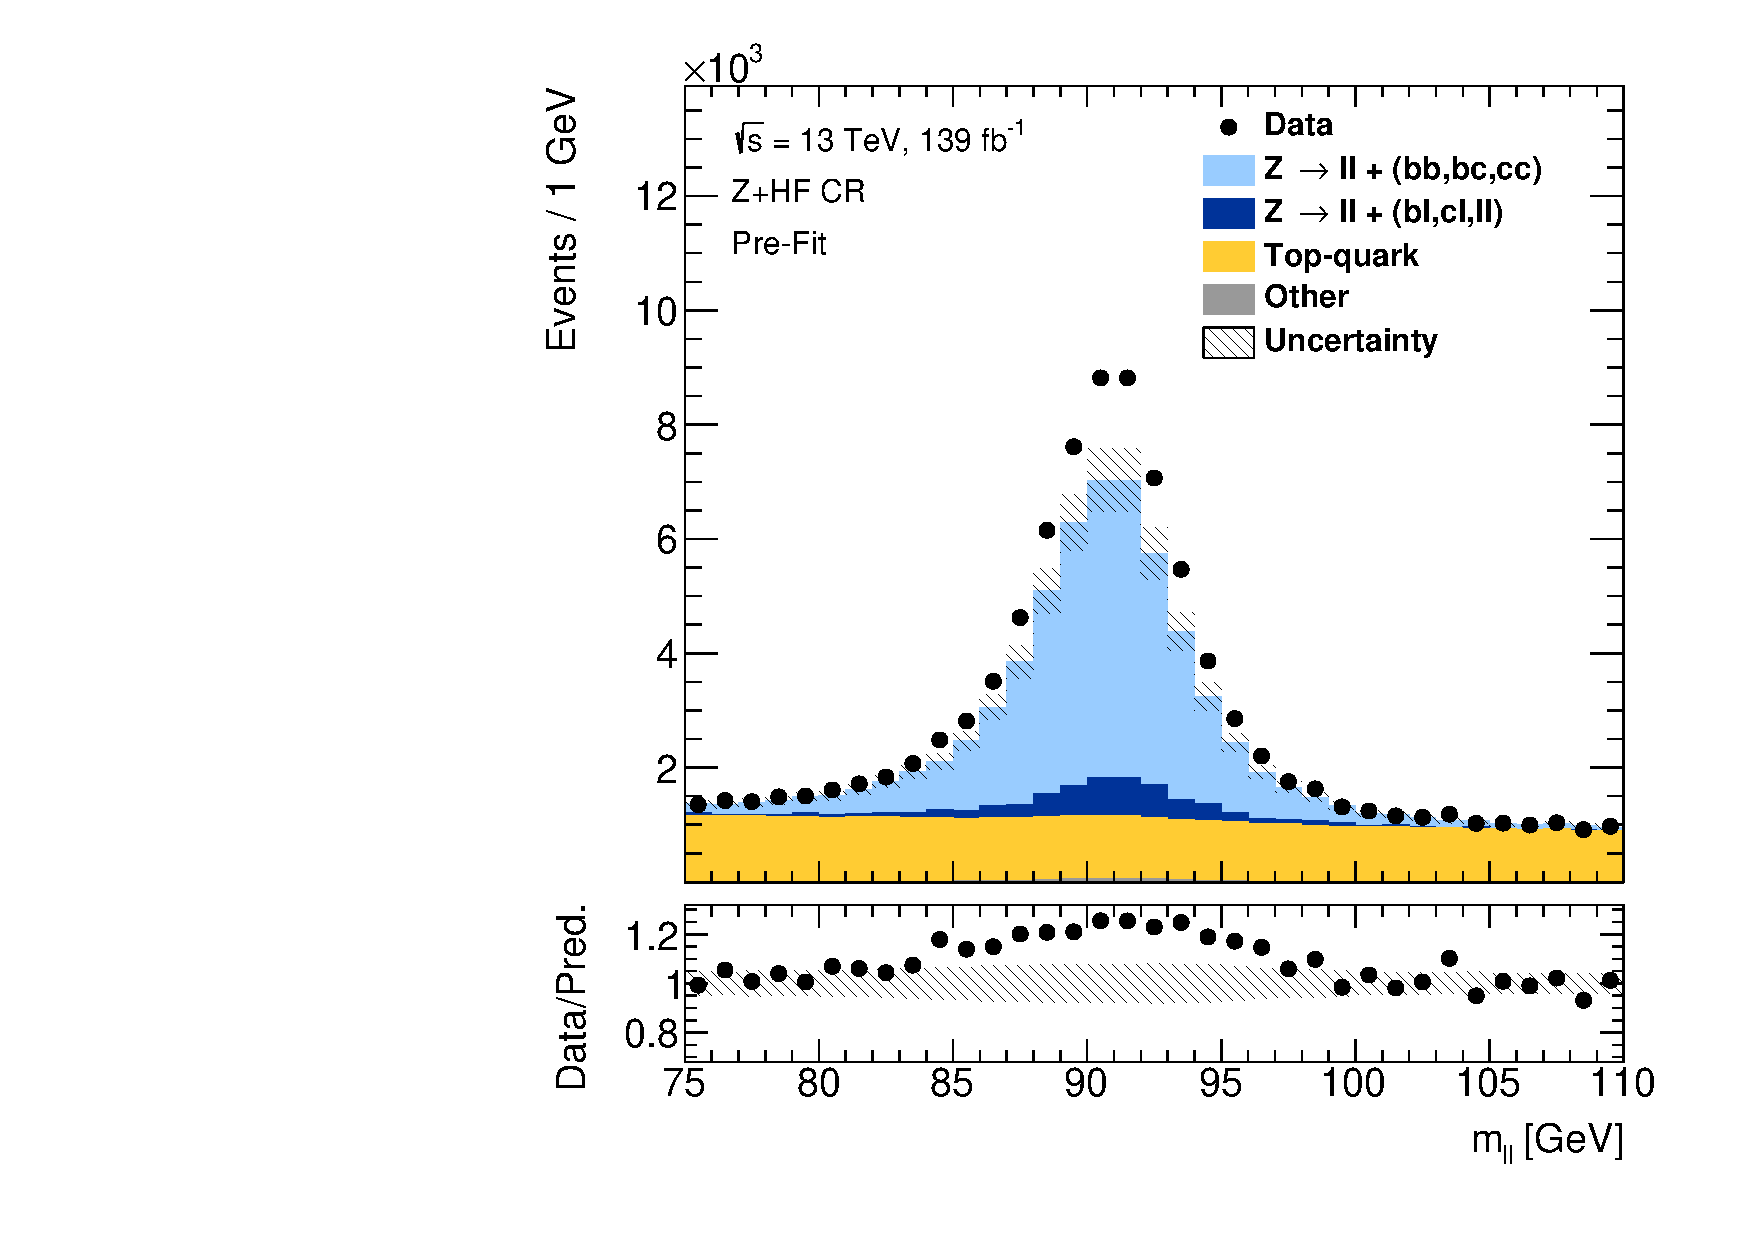
\includegraphics[width=\textwidth]{zhfcr/Region_BMin0_incJet1_Y2015_DZllbbCR_T2_L2_distmLL_J2_Prefit_fixed}
    \subcaption{Pre-fit}
    \label{fig:zcr_mll_prefit}
  \end{subfigure}\hfill%
  \begin{subfigure}{.485\textwidth}
    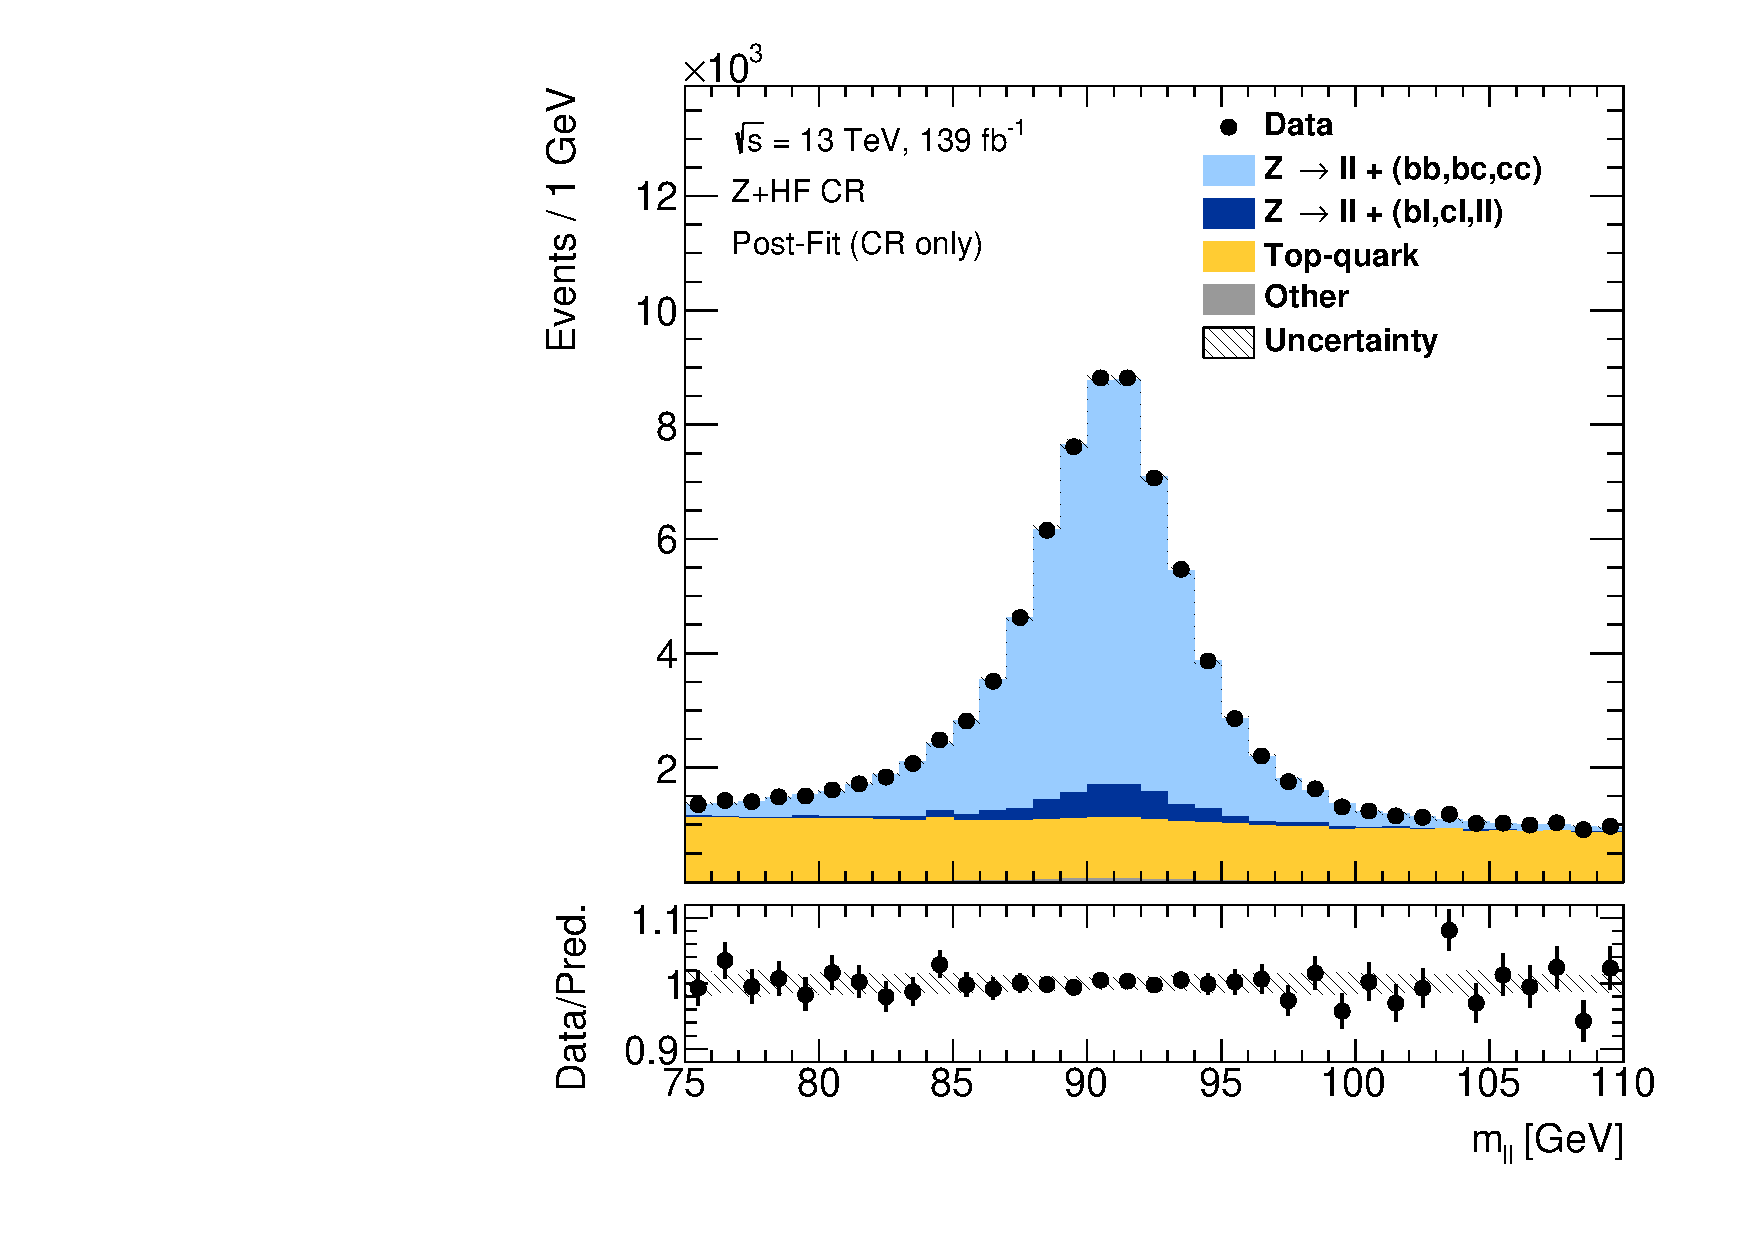
\includegraphics[width=\textwidth]{zhfcr/Region_BMin0_incJet1_Y2015_DZllbbCR_T2_L2_distmLL_J2_GlobalFit_conditionnal_mu0_fixed}
    \subcaption{Post-fit (\ZHF control region only)}
    \label{fig:zcr_mll_postfit}
  \end{subfigure}

  \caption{Distribution of the invariant di-lepton mass for the
    combination of electron- and muon-channel in the Z+HF control
    region before (a) and after (b) the likelihood fit restricted to
    the control region. The contribution of \Zjets is sub-divided into
    cases where both $b$-jet candidates are matched to heavy flavour
    quarks ($b$ or $c$) and cases where at most one candidate is
    matched to heavy flavour quarks at generator-level. The
    uncertainty includes all statistical and systematic
    uncertainties.}
\end{figure}

% ATLAS_norm_Zhf    1.3856e+00 +/-  1.19e-01
% ATLAS_norm_ttbar    9.7290e-01 +/-  3.92e-02
% Included in the SR fits: Systematic uncertainties are introduced at a later stage...
The \ZHF control region is later included in the likelihood fits that
are used to extract the \HH signals. Systematic uncertainties and the
combined fit model will be discussed in detail
in~\Cref{sec:uncertainties,sec:statistical_analysis}. Perform fits of
the control region only, the normalisation factors of \ZHF
are~\num{1.39 \pm 0.12} and for \ttbar~\num{0.97 \pm 0.04}. The
abundance of di-leptonic \ttbar in the control region provides
stringent constraints on the normalisation of the \ttbar background in
addition to constraining \ZHF. The post-fit event yields and \mll
distribution is shown in~\Cref{tab:zcr_postfit_yields}
and~\Cref{fig:zcr_mll_postfit}, respectively.

%%% Local Variables:
%%% mode: latex
%%% TeX-master: "../../phd_thesis"
%%% End:
